\documentclass[10pt,oneside]{article}

\usepackage{amsfonts}
\usepackage{amsmath}
\usepackage{amssymb}
\usepackage{dsfont}
\usepackage{bm}

\usepackage{epsf}
\usepackage{epsfig}
\usepackage{graphicx}
\usepackage{wrapfig} \usepackage{subfig}

\usepackage{enumerate}
\usepackage{listings}

\usepackage{setspace}
\usepackage{geometry}
\usepackage{fancyhdr}
%\usepackage{soul} % cross out text

\usepackage[latin2]{inputenc}
% \usepackage{times} % ez kiszedi a t1enc raszteressgt, de valami ms betu"tpust
% hasznl
\usepackage{lmodern} % ez eltu"nteti a raszteressget s mg jk is a betu"k
% \usepackage[magyar]{babel}
\usepackage{t1enc}

% \usepackage[T1]{fontenc}

\usepackage[usenames]{color}
% \usepackage[colorlinks]{hyperref} \usepackage{showkeys}

% \onehalfspacing
\usepackage{indentfirst}
% \frenchspacing

\geometry{left=2.5cm,right=2.5cm,top=3.0cm,bottom=2.5cm}

\pagestyle{fancy}
\lhead{Bayesian parameter estimation}
\chead{ }
\rhead{\thepage}

\lfoot{ }
\cfoot{ }
\rfoot{P\'{e}ter K\'{o}m\'{a}r, \the\year}


\renewcommand{\headrulewidth}{0.4pt}
\renewcommand{\footrulewidth}{0.0pt}



% \numberwithin{equation}{section} \numberwithin{figure}{section}
% \numberwithin{table}{section}

\author{Peter Komar}
\title{Methods of Bayesian Parameter Estimation}
\date{\today}





\begin{document}
\newcommand{\bel}{\begin{equation}}
\newcommand{\eel}{\end{equation}}
\newcommand{\be}{\begin{equation*}}
\newcommand{\ee}{\end{equation*}}

\newcommand{\bal}{\begin{eqnarray}}
\newcommand{\eal}{\end{eqnarray}}
\newcommand{\ba}{\begin{eqnarray*}}
\newcommand{\ea}{\end{eqnarray*}}

\newcommand{\ket}[1]{| #1 \rangle}
\newcommand{\Ket}[1]{\left| #1 \right\rangle}
\newcommand{\bra}[1]{\langle #1 |}
\newcommand{\Bra}[1]{\left\langle #1 \right|}

\newcommand{\no}{\noindent}

\newcommand{\ev}[1]{\langle #1 \rangle}
\newcommand{\Ev}[1]{\left\langle #1 \right\rangle}
\newcommand{\Tr}{\text{Tr}\,}
\newcommand{\T}{^\top}
\newcommand{\+}{^\dagger}
\newcommand{\s}{^\ast}
\newcommand{\PP}{\mathcal{P}}
\newcommand{\eqE}{= \!\!\!\!\!^{{}^{E}}\,}

\renewcommand{\d}[1]{\!d #1 \;}

\newcommand{\bE}{{\mathbf E}}
\newcommand{\bB}{{\mathbf B}}
\newcommand{\bF}{{\mathbf F}}
\newcommand{\bJ}{{\mathbf J}}
\newcommand{\bv}{{\mathbf v}}
\newcommand{\eps}{\varepsilon}
\newcommand{\br}{\mathbf r}
\newcommand{\bk}{\mathbf k}
\newcommand{\hatx}{\hat{\mathbf{x}}}
\newcommand{\haty}{\hat{\mathbf{y}}}
\newcommand{\hatz}{\hat{\mathbf{z}}}

\renewcommand{\vec}[1]{{\bf #1}}
\newcommand{\mat}[1]{{\bf #1}}

\newcommand{\op}[1]{\mathbf{#1}}
\newcommand{\twovector}[2]{
	\left[
		\begin{array}{c}
		#1 \\
		#2
		\end{array}
	\right]
}
\newcommand{\threevector}[3]{
	\left[
		\begin{array}{c}
		#1 \\
		#2 \\
		#3
		\end{array}
	\right]
}
\newcommand{\fourvector}[4]{
	\left[
		\begin{array}{c}
		#1 \\
		#2 \\
		#3 \\
		#4
		\end{array}
	\right]
}
\newcommand{\fivevector}[5]{
	\left[
		\begin{array}{c}
		#1 \\
		#2 \\
		#3 \\
		#4 \\
		#5
		\end{array}
	\right]
}
\newcommand{\nvector}[2]{
	\left[
		\begin{array}{c}
		#1_1 \\
		#1_2 \\
		\vdots \\
		#1_#2
		\end{array}
	\right]
}
\newcommand{\ncovector}[2]{
	[#1_1\s, #1_2\s, \dots #1_#2\s]
}
\newcommand{\twobytwomatrix}[4]{
	\left[
		\begin{array}{cc}
		#1 & #2\\
		#3 & #4
		\end{array}
	\right]
}
\newcommand{\threebythreematrix}[9]{
	\left[
		\begin{array}{ccc}
		#1 & #2 & #3\\
		#4 & #5 & #6\\
		#7 & #8 & #9
		\end{array}
	\right]
}
\newcommand{\threebythreedeterminant}[9]{
	\left|
		\begin{array}{ccc}
		#1 & #2 & #3\\
		#4 & #5 & #6\\
		#7 & #8 & #9
		\end{array}
	\right|
}
\newcommand{\nbymmatrix}[3]{
	\left[ 
		\begin{array}{cccc}
		#1_{11}  & #1_{12} & \dots  & #1_{1 #2}\\
		#1_{21}  & #1_{22} &        &         \\
		\vdots   &         & \ddots & \vdots  \\
		#1_{#3 1}&         & \dots  & #1_{#3 #2}
		\end{array}
	\right]
}
\newcommand{\nbyndeterminant}[2]{
	\left|
		\begin{array}{cccc}
		#1_{11}  & #1_{12} & \dots  & #1_{1 #2}\\
		#1_{21}  & #1_{22} &        &         \\
		\vdots   &         & \ddots & \vdots  \\
		#1_{#2 1}&         & \dots  & #1_{#2 #2}
		\end{array}
	\right|
}


\newcommand{\argmax}[1]{\underset{#1}{\operatorname{arg}\operatorname{max}}\;}

%\thispagestyle{empty}
%\maketitle
 
%\newpage
%\tableofcontents


\lstset{
numbers=left, 
numberstyle=\small, 
numbersep=8pt, 
frame = single, 
language=Python, 
framexleftmargin=15pt
}


\subsection*{Solution 1 - Linear regression}
The model for $N$ data points is
\be
	P(\{y_i\}\,|\,\{x_i\}, a, c, \sigma^2) = \prod_{i=1}^N \frac{1}{\sqrt{2\pi \sigma^2}} \exp\left[-\frac{(y_i - (a x_i + c))^2}{2\sigma^2}\right] = [2\pi\sigma^2]^{\frac{N}{2}} \exp\left[-\frac{1}{2\sigma^2}\sum_{i=1}^N \left[y_i - (ax_i + c)\right]^2\right].
\ee
Let's choose a non-informative prior
\be
	P_0(a,c,\sigma^2) = \frac{\text{const.}}{\sigma^2},
\ee
and write the posterior as 
\be
	P(a,c,\sigma^2\,|\,\{y_i\}, \{x_i\}) = \frac{1}{Z} (\sigma^2)^{-\frac{N+2}{2}} \exp\left[-\frac{1}{2\sigma^2}\left[y_i - (ax_i + c)\right]^2\right].
\ee
The quadratic form under the exponential suggests that the following statistics are going to be useful:
\ba
	&& N = 7,\qquad \ev{x} = \frac{\sum_i x_i}{N} = 4.0, \qquad \ev{y} = \frac{\sum_i y_i}{N} =  8.047, \\
	&& \ev{x^2} = \frac{\sum_i x_i^2}{N} = 20.0, \qquad \ev{xy} = \frac{\sum_i x_i y_i}{N} = 38.119, \qquad \ev{y^2} = \frac{\sum_i y_i^2}{N} = 73.650.
\ea

\subsubsection*{MAP + Laplace}
The unnormalized log-posterior is
\be
	\log\tilde P = -\frac{N+2}{2}\log(\sigma^2) - \frac{1}{2\sigma^2}\sum_i \big[y_i - (ax_i + c)\big]^2.
\ee
Equating the first derivative with 0 results in the following equations
\ba
	0 = \partial_a \log\tilde P &=& \frac{1}{\sigma^2}\sum_i x_i\big[y_i - (ax_i + c)\big] \\
	0 = \partial_c \log\tilde P &=& \frac{1}{\sigma^2}\sum_i \big[y_i - (ax_i + c)\big] \\
	0 = \partial_{\sigma^2} \log\tilde P &=& -\frac{N+2}{2}\frac{1}{\sigma^2} + \frac{1}{2(\sigma^2)^2} \sum_i \big[y_i - (ax_i + c)\big]^2,
\ea
which we can solve to get the MAP estimators
\ba
	a_\text{MAP} &=& \frac{\ev{xy} - \ev{x}\ev{y}}{\ev{x^2} - \ev{x}^2} =  1.4825\\
	c_\text{MAP} &=& \ev{y} - \ev{x}a_\text{MAP} =  2.1172\\
	(\sigma^2)_\text{MAP} &=& \frac{1}{N+2} \sum_i \left[y_i - (a_\text{MAP} x_i + c_\text{MAP})\right]^2 = 0.07971
\ea
The second derivative of the log-posterior at the MAP point is
\ba
	\left.\partial_a\partial_a \log\tilde P\right|_\text{MAP} &=& -\frac{1}{\sigma_\text{MAP}^2} \sum_i x_i^2 = - \frac{N\ev{x^2}}{\sigma_\text{MAP}^2} 
	\\
	\left.\partial_a\partial_c \log\tilde P\right|_\text{MAP} &=& -\frac{1}{\sigma_\text{MAP}^2} \sum_i x_i = - \frac{N\ev{x}}{\sigma_\text{MAP}^2}
	\\
	\left.\partial_c\partial_c \log\tilde P\right|_\text{MAP} &=& -\frac{1}{\sigma_\text{MAP}^2} \sum_i 1 = - \frac{N}{\sigma_\text{MAP}^2}
	\\
	\left.\partial_{\sigma^2}\partial_{\sigma^2}\log\tilde P\right|_\text{MAP} &=& \frac{N+2}{2}\frac{1}{(\sigma^2_\text{MAP})^2} - \frac{\sum_i[y_i - (a_\text{MAP} x_i + c_\text{MAP})]^2}{(\sigma^2_\text{MAP})^3} = -\frac{N+2}{2(\sigma^2_\text{MAP})^2}
\ea
\ba
	\left.\partial_{\sigma^2}\partial_a\log\tilde P\right|_\text{MAP} &=& -\frac{1}{(\sigma_\text{MAP}^2)^2}\sum_i x_i\big[y_i - (ax_i + c)\big] = 0
	\\
	\left.\partial_{\sigma^2}\partial_c\log\tilde P\right|_\text{MAP} &=& -\frac{1}{(\sigma_\text{MAP}^2)^2}\sum_i \big[y_i - (ax_i + c)\big] = 0
\ea
where the last two mixed derivatives are zero because they are proportional to the first derivatives with respect to $a$ and $c$, which are zero at the MAP point. Now, we can construct the Hessian, and take the negative inverse to obtain the Laplace covariance matrix
\ba
	\nabla\nabla \log \tilde P &=& -\frac{N}{\sigma_\text{MAP}^2}
	\threebythreematrix
	{\ev{x^2}}{\ev{x}}{0} 
	{\ev{x}}{1}{0} {0}{0}
	{\frac{N+2}{2N\sigma_\text{MAP}^2}}
	\\
	\text{Cov}_\text{L}\threevector{a}{c}{\sigma^2} = \left[-\nabla\nabla \log \tilde P\right]^{-1} &=& \frac{\sigma_\text{MAP}^2}{N}
	\threebythreematrix
	{\frac{1}{\ev{x^2} - \ev{x}^2}}{-\frac{\ev{x}}{\ev{x^2} - \ev{x}^2}}{0}
	{-\frac{\ev{x}}{\ev{x^2} - \ev{x}^2}}{\frac{\ev{x^2}}{\ev{x^2} - \ev{x}^2}}{0}
	{0}{0}{\frac{2N\sigma_\text{MAP}^2}{N+2}},
\ea
which provides the Laplace standard deviations and correlations
\ba
	\text{std}_\text{L}(a) &=& \sqrt{\frac{\sigma^2_\text{MAP}}{N} \frac{1}{\ev{x^2} - \ev{x}^2}} = 0.0534\\
	\text{std}_\text{L}(c) &=& \sqrt{\frac{\sigma^2_\text{MAP}}{N} \frac{\ev{x^2}}{\ev{x^2} - \ev{x}^2}} = 0.2386\\
	\text{corr}_\text{L}(a,c) &=& \frac{\text{cov}_\text{L}(a,c)}{\sqrt{\text{std}_\text{L}(a) \text{std}_\text{L}(c)}} = -\frac{\ev{x}}{\sqrt{\ev{x^2}}} = -0.89443\\
	\text{std}_L(\sigma^2) &=& \sqrt{\frac{2}{N+2}} \sigma^2_\text{MAP} = 0.0376
\ea

\subsubsection*{MCMC}
Let's construct the STAN code for the model.
\begin{lstlisting}[language={}]
data {
    int<lower=1> N;
    real x[N];
    real y[N];
}
parameters {
    real a;
    real c;
    real<lower=0> sigma2;
}
model {
    target += -log(sigma2);
    for (i in 1:N){
        target += normal_lpdf(y[i] | a * x[i] + c, sqrt(sigma2));
    }
}
\end{lstlisting}
Running sampling with STAN's NUTS algorithm over 4 chains, each with 100,000 iterations, the first half of each chain is dropped, and every 10th (thin=10) of the remaining constitutes 20,000 MCMC samples yielding the following approximations of means, medians, standard deviations and correlation of $a, c$ and $\sigma^2$:
\ba
	&&
	\mathbb{E}(a) \approx 1.482,\qquad 
	\text{median}(a) \approx 1.482, \\
	&& 
	\mathbb{E}(c) \approx 2.119,\qquad 
	\text{median}(c) \approx 2.120\\
	&& 
	\mathbb{E}(\sigma^2) \approx 0.2377,\qquad 
	\text{median}(\sigma^2) \approx 0.1639\\
	&&
	\text{std}(a) \approx 0.0920,\qquad 
	\text{std}(c) \approx 0.4130, \qquad
	\text{std}(\sigma^2) \approx 0.2828\\
	&&
	\text{corr}(a,c) = \frac{\text{cov}(a, c)}{\sqrt{\text{std}(a) \text{std}(c)}} \approx -0.8908,\qquad \text{corr}(a,\sigma^2) \approx 0.03771,\qquad \text{corr}(c,\sigma^2) \approx -0.03118
\ea

\subsubsection*{Exact}
The model can be cast into the general form of linear regression (See Appendix) with the following definitions,
\be
	K = 2, \qquad b = \twovector{a}{c},\qquad X = \fourvector{x_1\quad 1}{x_2\quad 1}{\vdots\qquad \vdots}{x_N\quad 1},\qquad y = \nvector{y}{N}.
\ee
After plugging in the data $\{x_i\},\,\{y_i\}$, we can calculate the following intermediate results
\ba
	\Lambda &=& \left[\frac{X\T X}{N}\right]^{-1} = \twobytwomatrix{0.25}{-1.00}{-1.00}{5.00},\\
	\bar b &=& \twovector{\bar a}{\bar c} = \frac{\Lambda X\T y}{N} = \twovector{1.4825}{2.1171},\\
	\bar v &=& \frac{(y - X\bar b)\T (y - X\bar b)}{N} = 0.10248.
\ea
Expectation values are
\ba
	&&\mathbb{E}(a) = \text{mode}(a) = \text{media}(a) = \bar a = 1.4825 \\
	&&\mathbb{E}(c) = \text{mode}(c) = \text{media}(c) = \bar c = 2.1171 \\
	&&\mathbb{E}(\sigma^2) = \frac{N\bar v}{N - K - 2} = 0.23912,\qquad \text{mode}(\sigma^2) = \frac{N\bar v}{N - K + 3} = 0.08967
\ea
Variance of $b$, standard deviation of $\sigma^2$ are
\be
	\text{Var}(b) = \frac{\bar v \Lambda}{N-K-2} = \twobytwomatrix{0.00855}{-0.03416}{-0.03416}{0.17080},\qquad \text{std}(\sigma^2) = \frac{\sqrt{2}N\bar v}{(N - K - 2)\sqrt{N- K - 4}} = 0.33817,
\ee
and the standard deviation and correlation of $a$ and $c$ are
\be
	\text{std}(a) = \sqrt{[\text{Var}(b)]_{1,1}} = 0.09241,\qquad 
	\text{std}(c) = \sqrt{[\text{Var}(b)]_{2,2}} = 0.41328,\qquad
	\text{corr}(a,c) = \frac{\Lambda_{1,2}}{\sqrt{\Lambda_{1,1} \Lambda_{2,2}}} = -0.89443,
\ee
and the correlation between $\sigma^2$ and $a$ or $c$ is exactly 0, as for all linear regression models with assumed uniform $\sigma^2$.

\newpage
\subsubsection*{Comparison}
We plot the marginals of $a, c$ and $\sigma^2$, and the joint marginal of $(a,c)$. MAP + Laplace  underestimates $\sigma^2$ and the uncertainties of $a$ and $c$.
\begin{figure}[h]
\centering
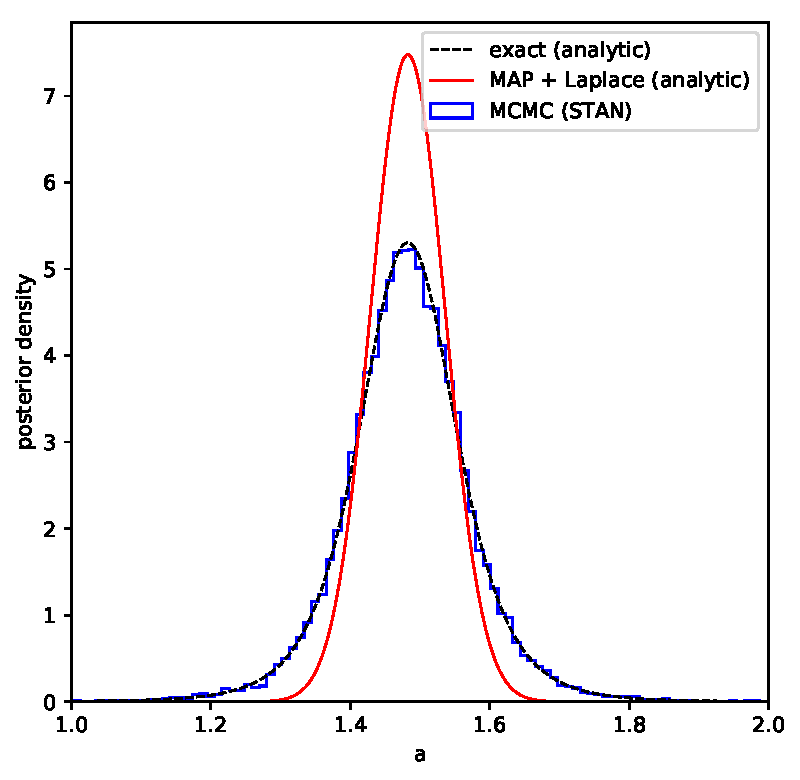
\includegraphics[width=0.49\textwidth]{P1_a_posterior.pdf}
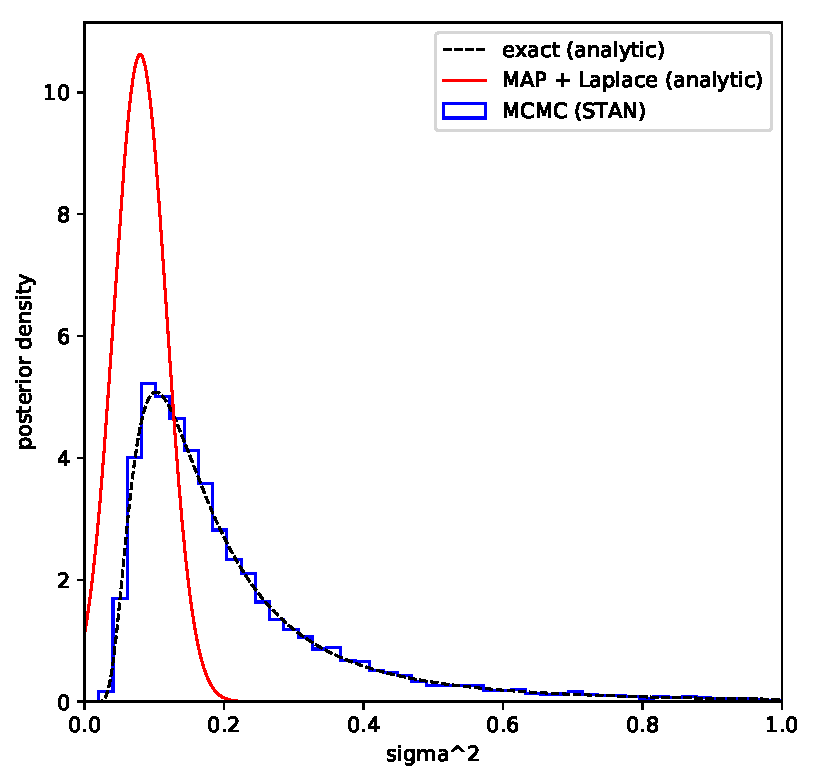
\includegraphics[width=0.49\textwidth]{P1_sigma2_posterior.pdf}
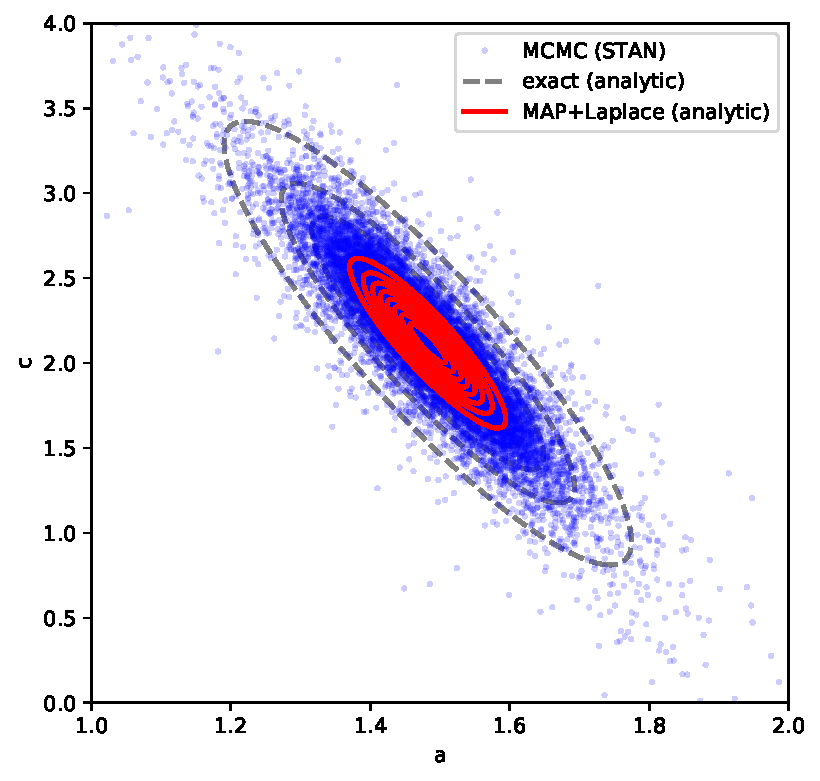
\includegraphics[width=0.49\textwidth]{P1_ac_joint_posterior.pdf}
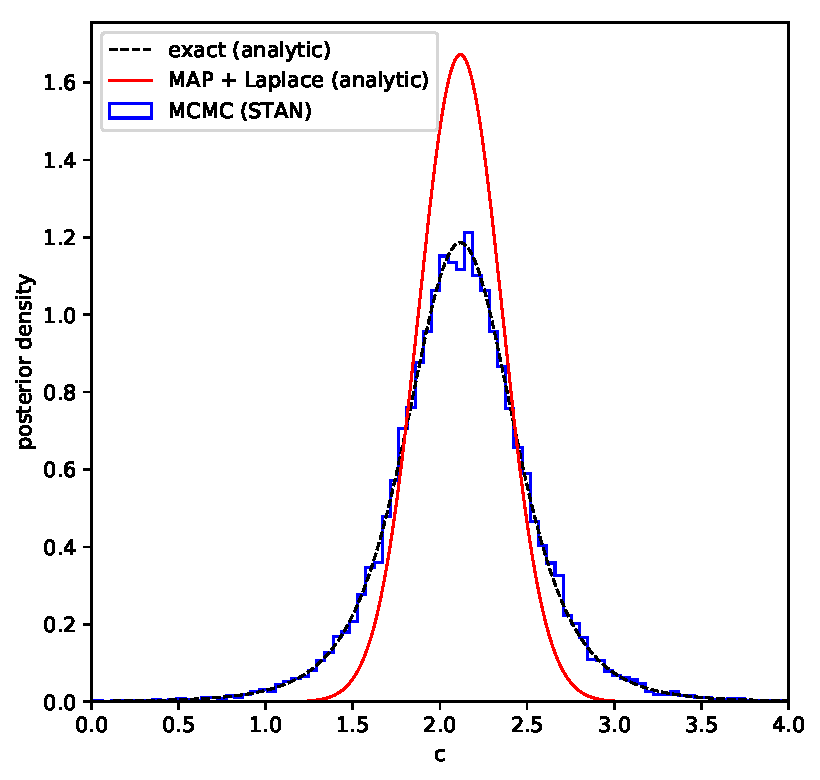
\includegraphics[width=0.49\textwidth]{P1_c_posterior.pdf}
\end{figure}



\newpage
\subsection*{Solution 2 - Negative binomial}
We assume that the number of failures $r$ is picked before all experiments, it is not generated by a probabilistic distribution. The only data is $k$, the number of successes, which is generated by a negative binomial distribution,
\be
	P(k\,|\,p) = {k + r - 1 \choose k} p^k (1-p)^r.
\ee
Let's use a non-informative prior for $p$:
\be
	P_0(p) = \frac{\text{const.}}{p(1-p)},
\ee
where const. is the appropriate normalization factor in a plausible region $0 < p_\text{low} \leq p < p_\text{high} < 1$. Now, the posterior of $p$ can be written as 
\ba
	P(p\,|\,k) &=& \text{const.}\times P_0(p) \times P(k\,|\,p) = \frac{1}{Z}\, p^{k-1}\, (1-p)^{r-1}.
\ea
The unnormalized log-posterior is
\be
	\log \tilde P(p\,|\,k) = (k-1)\log(p) + (r-1)\log(1-p).	
\ee


\subsubsection*{MAP + Laplace}
Equating the first derivative of the log-posterior with zero yields the MAP estimate:
\be
	0 = \partial_p \log\tilde P = \frac{k-1}{p} - \frac{r-1}{1-p} \qquad \Rightarrow \qquad p_\text{MAP} = \frac{k-1}{k+r -2} = 0.83333
\ee
The second derivative of, at the MAP point, can be used to calculate the Laplace standard deviation:
\be
	\left.\partial_p^2 \log\tilde P\right|_\text{MAP} = -\frac{k-1}{p_\text{MAP}^2} - \frac{r-1}{(1-p_\text{MAP})^2}\qquad\Rightarrow \qquad \text{std}_\text{L}(p) = \sqrt{-\left[\left.\partial_p^2 \log\tilde P\right|_\text{MAP}\right]^{-1}} = 0.07607
\ee

\subsubsection*{MCMC}
Let's construct the STAN code for the model.
\begin{lstlisting}[language={}]
data {
    int<lower=1> r;  // number of failures
    int<lower=1> k;  // number of successes
}
parameters {
    real<lower=0, upper=1> p;  // success probability
}
model {
    target += (k - 1) * log(p) + (r - 1) * log(1 - p);  // log-posterior
}
\end{lstlisting}

Although $r$ is not a probabilistic variable, it still works as an input to STAN, so it needs to be listed under ``data'' (line 2). We set a minimal allowed value for $k$ to 1 (line 3), because otherwise the posterior is not normalizable over $0<p<1$, which throws STAN off. Line 9 defines the unnormalized log-posterior.

After sampling with STAN's NUTS algorithm, 4 chains, 2000 iterations each, dropping the first 1000, and not thinning the remaining (thin = 1), we obtain the following mean, median and standard deviation estimates
\ba
	\mathbb{E}(p) & \approx & 0.80759 \\
	\text{median}(p) & \approx & 0.81525 \\
	\text{std}(p) & \approx & 0.07577
\ea

\subsubsection*{Exact}
We apply the limits $p_\text{low} \rightarrow 0$, $p_\text{high}\rightarrow 1$. The analytical formula for the normalization constant $Z$ can be found by integrating over $0 < p < 1$:
\be
	Z = \intop_0^1 \d{p} p^{k-1} (1-p)^{r-1} = \mathcal{B}(k, r) = \frac{\Gamma(k)\Gamma(r)}{\Gamma(k+r)} = \frac{(k-1)! (r-1)!}{(k+r-2)!},
\ee
where $\mathcal{B}$ is the beta function. This allows us to write the posterior as
\be
	P(p\,|\,k) = \frac{p^{k-1} p^{r-1}}{\mathcal{B}(k,r)} =: \frac{p^{\alpha-1} p^{\beta-1}}{\mathcal{B}(\alpha,\beta)}  = \text{Beta}(p\,|\, \alpha, \beta),
\ee
which is the beta distribution for $\alpha = k$ and $\beta = r$. The formulas for mean, median, mode, and standard deviation are known:
\ba
	\mathbb{E}(p) &=& \frac{\alpha}{\alpha + \beta} = \frac{k}{k + r} = 0.80769 \\ 
	\text{median}(p) &\approx& \frac{\alpha - \frac{1}{3}}{\alpha + \beta - \frac{2}{3}} = 0.81579 \\
	\text{mode}(p) &=& \frac{\alpha -1}{\alpha + \beta -2} = 0.83333 \\
	\text{std}(p) &=& \sqrt{\frac{\alpha\beta}{(\alpha + \beta)^2(\alpha + \beta + 1)}} = 0.07585
\ea

\subsubsection*{Comparison}
MAP + Laplace method approximates the posterior with a Gaussian centered at the mode. Our MCMC run produced 4000 samples, the histogram of which can be plotted. The exact solution resulted in the beta distribution, which is readily implemented in Python's \texttt{scipy.stats.beta}. Let's compare their estimates graphically.
\begin{figure}[h]
\centering
	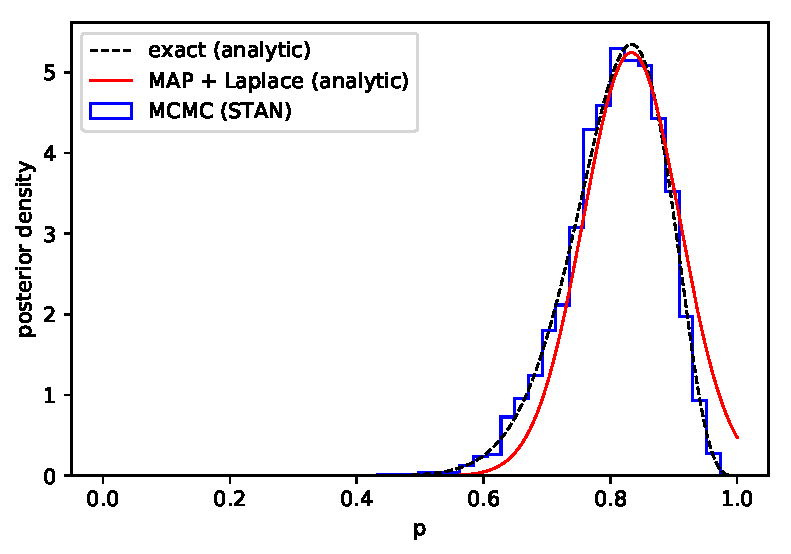
\includegraphics[width=0.6\textwidth]{P2_p_posterior.pdf}
\end{figure}


\newpage
\subsection*{Solution 3 - Normal}
From the data $\{x_i\}_{i=1}^N$, let's calculate two important statistics, the empirical mean and empirical variance:
\be
	N = 7,\qquad \bar x = \frac{\sum_i x_i}{N} = 114.71,\qquad \bar v = \frac{\sum_i (x_i - {\bar x})^2}{N} = 103.35
\ee
Each data point is assumed to come from a normal distribution, independent from the other data points. The resulting likelihood is 
\be
	P(\{x_i\}\,|\,\mu, \sigma^2) = \prod_{i=1}^N \frac{1}{\sqrt{2\pi \sigma^2}} \exp\left[-\frac{(x_i - \mu)^2}{2\sigma^2}\right] = \left[2\pi \sigma^2\right]^{-\frac{N}{2}} \exp\left[-\frac{1}{2\sigma^2}\sum_{i=1}^N (x_i - \mu)^2\right]
\ee
We use a non-informative prior for $\mu$ and $\sigma^2$,
\be
	P_0(\mu, \sigma^2) = P_0(\mu) \times P_0(\sigma^2) = \text{const.} \times \frac{\text{const.}}{\sigma^2} = \frac{\text{const.}}{\sigma^2},
\ee
where the constants are appropriately chosen to normalize the prior distribution on plausible a interval, $\mu_\text{low} \leq \mu \leq \mu_\text{high}$, and $0 < \sigma^2_\text{low} \leq \sigma^2 \leq \sigma^2_\text{high}$.

The posterior can be written as 
\be
	P(\mu, \sigma^2\,|\,\{x_i\}) = \text{const.} \times P_0(\mu, \sigma^2) \times P(\{x_i\}\,|\, \mu, \sigma^2) = \frac{1}{Z} (\sigma^2)^{-\frac{N+2}{2}} \exp\left[-\frac{1}{2\sigma^2}\sum_{i=1}^N (x_i - \mu)^2\right],
\ee
and the unnormalized log-posterior is
\be
	\log \tilde P(\mu, \sigma^2\,|\,\{x_i\}) = -\frac{N + 2}{2} \log(\sigma^2) - \frac{1}{2\sigma^2} \sum_i (x_i - \mu)^2.
\ee

\subsubsection*{MAP + Laplace}
Setting the first derivatives of the log-posterior to zero yields the MAP estimates:
\ba
	0 &=& \partial_\mu \log\tilde P = \frac{1}{\sigma^2} \sum_i (x_i - \mu) \qquad \Rightarrow \quad \mu_\text{MAP} = \frac{\sum_i x_i}{N} = \bar x = 114.71\\
	0 &=& \partial_{\sigma^2} \log\tilde P = -\frac{N+2}{2\sigma^2} + \frac{1}{2(\sigma^2)^2}\sum_i(x_i - \mu)^2 \qquad \Rightarrow \quad (\sigma^2)_\text{MAP} = \frac{\sum_i(x_i - \mu_\text{MAP})^2}{N+2} = \frac{N\bar v}{N+2} = 80.381
\ea
The second-oder derivatives at the MAP point are
\ba
	\left.\partial_\mu\partial_\mu \log\tilde P\right|_\text{MAP} &=& \left.-\frac{N}{\sigma^2}\right|_\text{MAP} =  - \frac{N+2}{\bar v} \\
	\left.\partial_\mu\partial_{\sigma^2} \log\tilde P\right|_\text{MAP} &=& \left.-\frac{1}{\sigma^2}\sum_i(x_i - \mu)\right|_\text{MAP} = 0\\
	\left.\partial_{\sigma^2}\partial_{\sigma^2} \log\tilde P\right|_\text{MAP} &=& \left.\frac{N+2}{2(\sigma^2)^2} - \frac{\sum_i (x_i - \mu)^2}{(\sigma^2)^3}\right|_\text{MAP}= \frac{N+2}{2(\sigma^2_\text{MAP})^2} - \frac{N\bar v}{(\sigma^2_\text{MAP})^3} = -\frac{(N+2)^3}{2(N\bar v)^2}
\ea
The Laplace covariance matrix of $(\mu, \sigma^2)$ is the negative inverse of the Hessian at the MAP point:
\ba
	\text{Cov}_\text{L}\twovector{\mu}{\sigma^2} = \left[\left. -\nabla\nabla\log \tilde P\right|_\text{MAP}\right]^{-1} = \twobytwomatrix{\frac{N+2}{\bar v}}{0}{0}{\frac{(N+2)^3}{2(N\bar v)^2}}^{-1} = \twobytwomatrix{\frac{\bar v}{N+2}}{0}{0}{\frac{2(N\bar v)^2}{(N+2)^3}},
\ea
from which, we can extract the formulas for the Laplace standard deviations, and correlation
\ba
	\text{std}_\text{L}(\mu) = \sqrt{\frac{\bar v}{N+2}} = 3.3887, \quad \text{std}_\text{L}(\sigma^2) = \sqrt{\frac{2}{N+2}} \frac{N\bar v}{N+2} = 37.892, \quad \text{corr}_\text{L}(\mu, \sigma^2) = \frac{\text{cov}_\text{L}(\mu, \sigma^2)}{\text{std}_\text{L}(\mu)\,\text{std}_\text{L}(\sigma^2)} = 0.
\ea

To estimate the probability that $\mu < 100$, we recall that the Laplace approximation assumes a Gaussian shape for the posterior, centered at the MAP point. For $\mu$, this is
\be
	P(\mu\,|\,\{x_i\}) \approx \text{Norm}(\mu\,|\,\mu_\text{MAP}, \text{std}_\text{L}(\mu)) = \text{Norm}(\mu\,|\,114.71,\, 3.3887),
\ee
and the probability of $\mu < 100$ is estimated as 
\be
	P(\mu < 100\,|\,\{x_i\}) = \intop_{-\infty}^{100} \d{\mu} P(\mu\,|\,\{x_i\})\;\approx\; \text{cdf-Norm}(100\,|\, 114.71,\,3.3887) = 7\times 10^{-6},
\ee
where cdf-Norm is the cumulative distribution function of a the normal distribution, readily implemented in Python's \texttt{scipy.stats.norm} as \texttt{cdf}.


\subsubsection*{MCMC}
Let's construct the STAN code for the model.
\begin{lstlisting}[language={}]
data {
    int<lower=1> N;
    real x[N];
}
parameters {
    real mu;
    real<lower=0> sigma2;
}
model {
    target += -log(sigma2);
    for (i in 1:N){
        target += normal_lpdf(x[i] | mu, sqrt(sigma2));
    }
}
\end{lstlisting}

The ``data'' section includes $N$ in line 2, because STAN needs to know how many $x_i$ values to expect. In line 11, we loop over the input $x_i$ values and add the log-probability contribution of each, which is readily implemented in STAN's \texttt{normal\_lpdf(x | mu, sigma)} function (See section 54.1 in STAN manual).

Running sampling with STAN's NUTS algorithm over 4 chains, each with 100,000 iterations, the first half of each chain is dropped, and every 10th (thin=10) of the remaining constitutes 20,000 MCMC samples yielding the following approximates of means, medians, standard deviations and correlation of $\mu$ and $\sigma^2$:
\ba
	&&\mathbb{E}(\mu) \approx 114.69,\qquad 
	\text{median}(\mu) \approx 114.69, \qquad 
	\text{std}(\mu) \approx 5.0706,\\
	&& \mathbb{E}(\sigma^2) \approx 179.39,\qquad
	\text{median}(\sigma^2) \approx 135.87, \qquad 
	\text{std}(\sigma^2) \approx 164.42, \\
	&& \text{corr}(\mu, \sigma^2) = \frac{\text{cov}(\mu,\sigma^2)}{\text{std}(\mu) \text{std}(\sigma^2)} \approx 0.014.
\ea

The probability of $\mu < 100$, can be estimated by counting what fraction of the MCMC samples $\{\mu^{(t)}\,: t=1,2,\ldots T\}$) is below 100, this turned out to be
\be
	P(\mu < 100) \approx \frac{\#\left[\mu^{(t)} < 100\right]}{T} = \frac{117}{20000} = 5.9\times 10^{-3}.
\ee


\subsubsection*{Exact}
The analytical formula for the normalization constant $Z$ can be calculated with the integral over $\mu \in(-\infty, +\infty)$, $\sigma^2\in [0, \infty)$:
\be
	Z 
	= \intop_0^\infty\d{\sigma^2} (\sigma^2)^{-\frac{N+2}{2}} \intop_{-\infty}^{+\infty}\d{\mu}  \exp\left[-\frac{\sum_i (x_i - \mu)^2}{2\sigma^2}\right],
\ee
where the $\mu$-integral can be written as
\ba
	\intop_{-\infty}^{+\infty}\d{\mu}  \exp\left[-\frac{N\mu^2 - 2\mu\sum_i x_i + \sum_i x_i^2}{2\sigma^2}\right] = \exp\left[-\frac{N\bar v}{2\sigma^2}\right] \underbrace{\intop_{-\infty}^{+\infty}\d{\mu} \exp\left[-\frac{N(\mu - \bar x)^2}{2\sigma^2}\right]}_{\sqrt{2\pi\sigma^2 / N}},
\ea
and $Z$ can be written as
\be
	Z 
	= 
	\sqrt{\frac{2\pi}{N}} \intop_0^\infty\d{\sigma^2} (\sigma^2)^{-\frac{N+1}{2}} \exp\left[-\frac{N\bar v}{2\sigma^2}\right]
	=
	\sqrt{\frac{2\pi}{N}} \left(\frac{2}{N\bar v}\right)^{\frac{N-1}{2}} \underbrace{\intop_0^\infty \d{z} z^{\frac{N-3}{2}} \exp(-z)}_{\Gamma\left(\frac{N-1}{2}\right)},
\ee
where we introduced a new integration variable $z = \frac{N\bar v}{2\sigma^2}$, and substituted $\sigma^2 = \frac{N\bar v}{2z}$ and $d\sigma^2 = - \frac{N\bar v}{2z^2} dz$, and got rid of the minus sign by flipping the integration limits. Now we can write the normalized posterior as 
\be
	P(\mu, \sigma^2\,|\, \{x_i\}) = \frac{\sqrt{N}}{\sqrt{2\pi \sigma^2}} \frac{1}{\Gamma\left(\frac{N-1}{2}\right)} \left(\frac{N\bar v}{2}\right)^{\frac{N-1}{2}} (\sigma^2)^{-\frac{N-1}{2} - 1} \exp\left[-\frac{2\left(\frac{N\bar v}{2}\right) + N(\mu - \bar x)^2}{2\sigma^2}\right],
\ee
which we can identify with the normal-inverse-gamma distribution,
\be
	\text{N-IG}(\mu, \sigma^2\,|\,\mu_c, \lambda, \alpha, \beta) = \frac{\sqrt{\lambda}}{\sqrt{2\pi \sigma^2}}\frac{\beta^\alpha}{\Gamma(\alpha)} (\sigma^2)^{-\alpha - 1} \exp\left[-\frac{2\beta + \lambda((\mu - \mu_c)^2)}{2\sigma^2}\right],
\ee
with parameters $\mu_c = \bar x$, $\lambda = N$, $\alpha = \frac{N-1}{2}$ and $\beta = \frac{N\bar v}{2}$. The mean, mode, standard deviation and correlation are known
\ba
	&&\mathbb{E}(\mu) = \mu_c = \bar x = 114.71,\qquad 
	\text{mode}(\mu) = \mu_c = \bar x = 114.71, \\ 
	&&\text{std}(\mu) = \sqrt{\frac{\beta}{\lambda(\alpha - 1)}} = \sqrt{\frac{\bar v}{N-3}} = 5.0830,\\
	&& \mathbb{E}(\sigma^2) = \frac{\beta}{\alpha -1} = \frac{N\bar v}{N-3} = 180.86,\qquad
	\text{mode}(\sigma^2) = \frac{\beta}{\alpha + \frac{3}{2}} = \frac{N\bar v}{N+2} = 80.381, \\ 
	&&\text{std}(\sigma^2) = \frac{\beta}{(\alpha -1) \sqrt{\alpha -2}} = \frac{\sqrt{2}N\bar v}{(N-3)\sqrt{N-5}} = 144.69, \\
	&& \text{corr}(\mu, \sigma^2) = \frac{\text{cov}(\mu,\sigma^2)}{\text{std}(\mu) \text{std}(\sigma^2)} = 0.
\ea

To calculate the probability that $\mu < 100$, we need to find the marginal posterior distribution of $\mu$:
\be
	P(\mu\,|\,\{x_i\}) = \intop_0^\infty \d{\sigma^2} P(\mu, \sigma^2\,|\, \{x_i\}) = \sqrt{\frac{N}{2\pi}} \frac{\left(\frac{N\bar v}{2}\right)^{\frac{N-1}{2}}}{\Gamma\left(\frac{N-1}{2}\right)}\intop_0^\infty \d{\sigma^2} (\sigma^2)^{-\frac{N+2}{2}} \exp\left[-\frac{N\bar v + N(\mu - \bar x)^2}{2\sigma^2}\right]
\ee
The integral over $\sigma^2$ can be evaluated by introducing a new variable $z = \frac{N\bar v + N(\mu - \bar x)^2}{2\sigma^2}$, giving
\be
	\intop_0^\infty\d{\sigma^2}[\ldots] = \left[\frac{2}{N(\bar v + (\mu - \bar x)^2)}\right]^{\frac{N}{2}} \underbrace{\intop_0^\infty \d{z} z^{\frac{N}{2}-1} \exp(-z)}_{\Gamma(N/2)},
\ee
resulting in
\be
	P(\mu\,|\,\{x_i\}) 
	= 
	\frac{1}{\sqrt{\pi \bar v}} \frac{\Gamma\left(\frac{N}{2}\right)}{\Gamma\left(\frac{N-1}{2}\right)} \left[1 + \frac{(\mu - \bar x)^2}{\bar v}\right]^{-\frac{N}{2}} 
	=: 
	\frac{1}{\sqrt{\nu \pi s^2}} \frac{\Gamma\left(\frac{\nu +1}{2}\right)}{\Gamma\left(\frac{\nu}{2}\right)} \left[1 + \frac{(\mu - \mu_c)^2}{\nu s^2}\right]^{-\frac{\nu +1}{2}}
\ee
which is a (shifted and scaled) t-distribution with parameters $\nu = N-1$, $\mu_c = \bar x$ and $s = \sqrt{\bar v / (N-1)}$. The probability in question can now be directly calculated as the cumulative function of this t-distribution:
\be
	P(\mu < 100\,|\,\{x_i\}) \;=\; \text{cdf-t-dist}(100\,|\,\nu=N-1, \;\text{loc} = \bar x, \;\text{scale} = \sqrt{\bar v / (N-1)}) \; =\; 6.069\times 10^{-3}.
\ee
which is readily implemented in Python's \texttt{scipy.stats.t} as \texttt{cdf}.


\subsubsection*{Comparison}
Let's plot the estimated posterior marginals of $\mu$ and $\sigma^2$, and the contour plot of their joint posterior.
\begin{figure}[h]
\centering
	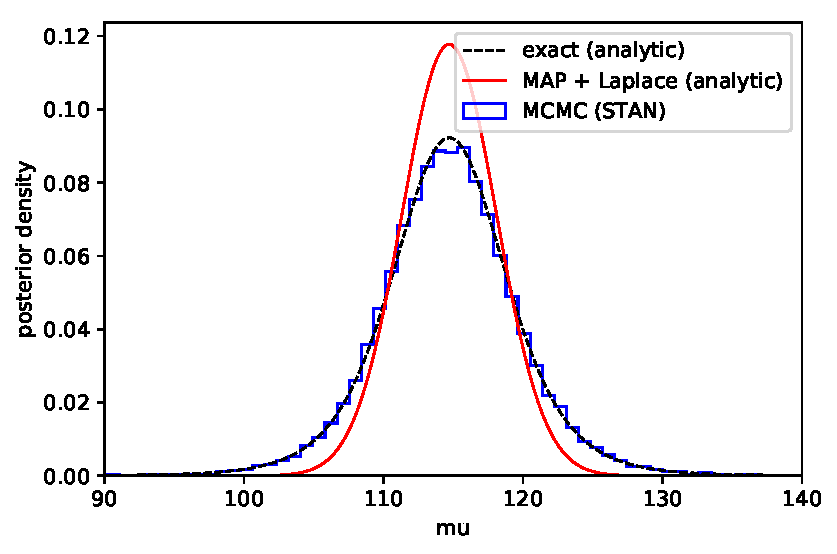
\includegraphics[width=0.49\textwidth]{P3_mu_posterior.pdf}
	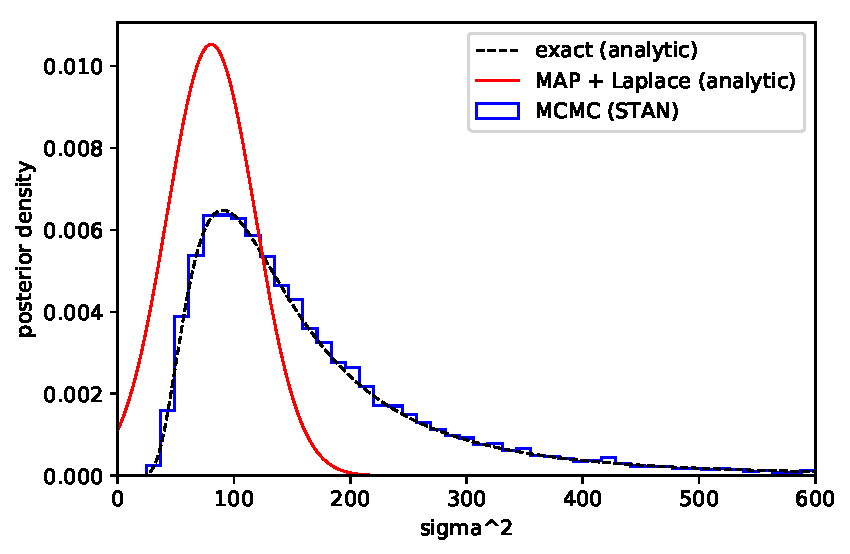
\includegraphics[width=0.49\textwidth]{P3_sigma2_posterior.pdf}
\end{figure}

\begin{figure}[h]
\centering
	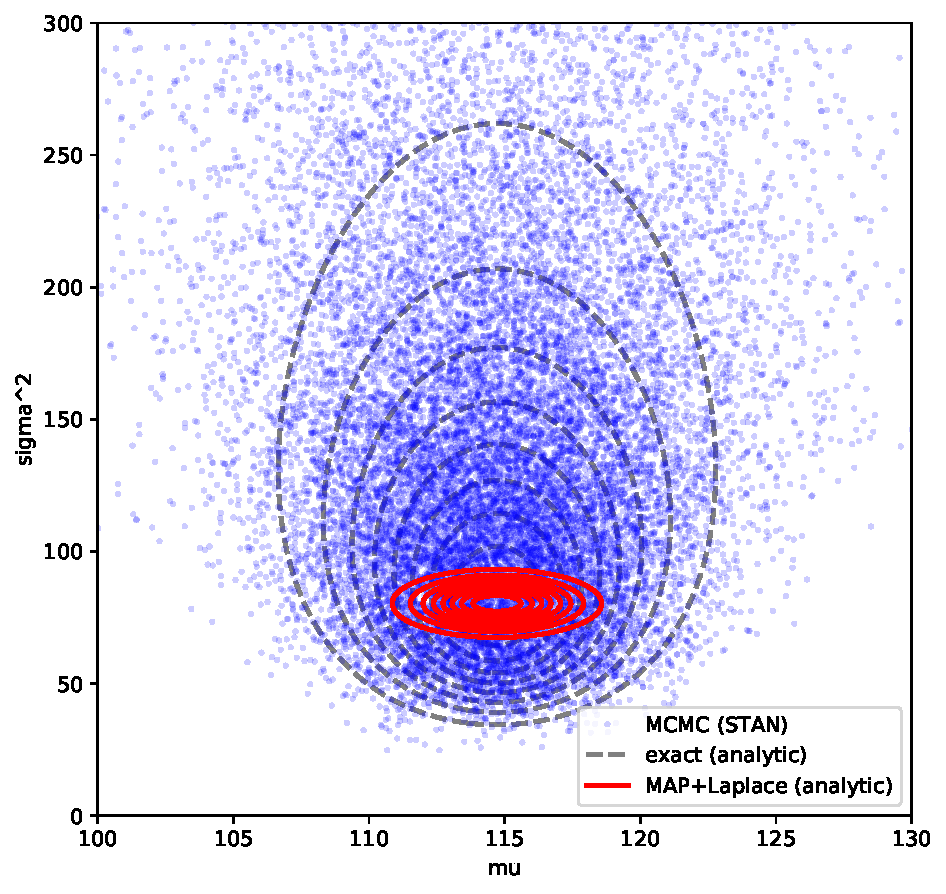
\includegraphics[width=0.40\textwidth]{P3_joint_posterior.pdf}
\end{figure}


\subsection*{Solution 4 - Fixed effect model}
Yields $\{y_{g,i}\}$ are indexed by group, $g\in\{A, B, C\}$, and a sequential index within the group $i \in \{1,2,\ldots n_g\}$, where $n_g$ is the number of values in group $g$. Let's define $G = \sum_g 1$, $N = \sum_g n_g$, i.e. the number of groups and the number of total data points, respectively. Each $y_{g,i}$ is assumed to be normally distributed around the corresponding group mean $\mu_g$,
\be
	P(y_{g,i}\,|\,\mu_g,\sigma^2) = \text{Norm}(y_{g,i}\,|\,\mu_g, \sigma^2) = \frac{1}{\sqrt{2\pi\sigma^2}}\exp\left[-\frac{(y_{g,i} - \mu_g)^2}{2\sigma^2}\right],
\ee
the product of these terms give the full likelihood
\be
	P(\{y_{g,i}\}\,|\,\{\mu_g\}, \sigma^2) = \prod_g \prod_{i=1}^{n_g}\text{Norm}(y_{g,i}\,|\,\mu_g, \sigma^2) = [2\pi\sigma^2]^{-\frac{N}{2}} \exp\left[-\frac{1}{2\sigma^2}\sum_g\sum_{i=1}^{n_g}(y_{g,i} - \mu_g)^2\right].
\ee
Using a non-informative prior,
\be
	P_0(\{\mu_g\}, \sigma^2) = P_0(\sigma^2) \prod_g P_0(\mu_g) = \frac{\text{const.}}{\sigma^2} \prod_g \text{const.} = \frac{\text{const.}}{\sigma^2},
\ee
results in the following posterior
\be
	P(\{\mu_g\}, \sigma^2\,|\,\{y_{g,i}\}) = \text{const.} \times P_0(\{\mu_g\}, \sigma^2)\times P(\{y_{g,i}\}\,|\,\{\mu_g\}, \sigma^2) = \frac{1}{Z} (\sigma^2)^{-\frac{N+2}{2}} \exp\left[-\frac{1}{2\sigma^2}\sum_g\sum_{i=1}^{n_g}(y_{g,i} - \mu_g)^2\right].
\ee
Let's calculate the following statistics from the data
\be
	G = 3,\qquad N = 13, \qquad \{\bar\mu_g\} = \Big\{\frac{1}{n_g}\sum_i y_{g,i}\Big\} = \threevector{\bar\mu_A}{\bar\mu_B}{\bar\mu_C} = \threevector{2507.5}{1569.8}{1337.7},\qquad \bar v = \frac{1}{N} \sum_g\sum_{i=1}^{n_g} (y_{g,i} - \bar \mu_g)^2 = 42817.0
\ee


\subsubsection*{MAP + Laplace}
The log-posterior is
\be
	\log\tilde P = -\frac{N+2}{2}\log(\sigma^2) - \frac{1}{2\sigma^2}\sum_g\sum_{i=1}^{n_g} (y_{g,i} - \mu_g)^2.
\ee
Setting the first derivatives to zero gives the MAP estimates
\ba
	0 = \partial_{\mu_g} \log\tilde P &=& \frac{1}{\sigma^2}\sum_{i=1}^{n_g} (y_{g,i} - \mu_g)
	\qquad \hspace{2cm} \Rightarrow \quad
	(\mu_{g})_\text{MAP} = \frac{1}{n_g}\sum_{i=1}^{n_g} y_{g,i} = \bar \mu_g\qquad \forall g
	\\
	0 = \partial_{\sigma^2}\log\tilde P &=& -\frac{N+2}{2\sigma^2} + \frac{\sum_g\sum_{i=1}^{n_g} (y_{g,i} - \mu_g)^2 }{2(\sigma^2)^2}
	\quad \Rightarrow \quad
	(\sigma^2)_\text{MAP} = \frac{\sum_{g,i} \big[y_{g,i} - (\mu_g)_\text{MAP}\big]^2}{N+2} = \frac{N\bar v}{N+2}
\ea
The second derivatives at the MAP point are
\ba
	\left.\partial_{\mu_g}\partial_{\mu_g} \log\tilde P\right|_\text{MAP} &=& - \frac{n_g}{\sigma^2} \qquad  \forall g
	\\
	\left.\partial_{\mu_g}\partial_{\mu_{g'}} \log\tilde P\right|_\text{MAP} &=& 0\qquad \text{if } g \neq g'
	\\
	\left.\partial_{\sigma^2}\partial_{\mu_g}\log\tilde P\right|_\text{MAP} &=& -\frac{1}{(\sigma^2)^2} \sum_i \big[y_{g,i} - (\mu_g)_\text{MAP}\big] = 0
	\\
	\left.\partial_{\sigma^2}\partial_{\sigma^2}\log\tilde P\right|_\text{MAP} &=& \frac{N+2}{2(\sigma^2)_\text{MAP}^2} - \frac{\sum_{g,i} [y_{g,i} - (\mu_g)_\text{MAP}]^2}{(\sigma^2)_\text{MAP}^3} = -\frac{N+2}{2((\sigma^2)_\text{MAP})^2} = -\frac{(N+2)^3}{2N^2\bar v^2},
\ea
Because the mixed derivatives are 0 at the MAP point, we can invert the Hessian ($\nabla\nabla \log\tilde P$) term by term, giving the following Laplace standard deviations
\be
	\text{std}_\text{L}(\mu_g) = \sqrt{\frac{\bar v}{N+2}}, \qquad 
	\text{std}_\text{L}(\sigma^2) = \sqrt{\frac{2}{N+2}}\frac{N\bar v}{N+2}.
\ee

To summarize, the MAP + Laplace estimates are
\ba
	\mu_A:&& (\mu_A)_\text{MAP} \pm \text{std}_\text{L}(\mu_A) = 2507.5 \pm 96.3\\
	\mu_B:&& (\mu_B)_\text{MAP} \pm \text{std}_\text{L}(\mu_B) = 1569.8 \pm 78.6\\
	\mu_C:&& (\mu_C)_\text{MAP} \pm \text{std}_\text{L}(\mu_C) = 1337.7 \pm 111.2\\
	\sigma^2:&& (\sigma^2)_\text{MAP} \pm \text{std}_\text{L}(\sigma^2) = 37108 \pm 13549
\ea

\subsubsection*{MCMC}
STAN can only handle rectangular arrays, and since $\{y_{g,i}\}$ cannot be reliably cast into such an array, we use an additional input: group labels, $l_j \in \{1,2,3\}$, signifying which group does the $j$th data point belong to. With this definition, our data is
\ba
	y = \{y_j\,:\,j=1,2,\ldots N\} &=& [2604, 2665, 2251, 2510, 1559, 1729, 1866, 1414, 1159, 1692, 1528, 1444, 1041]\\
	l = \{l_j\,:\,j=1,2,\ldots N\} &=& [1, 1, 1, 1, 2, 2, 2, 2, 2, 2, 3, 3, 3].
\ea
This allows us to run the following STAN code.
\begin{lstlisting}[language={}]
data {
    int<lower=1> G;  // number of groups
    int<lower=1> N;  // number of total data points
    int<lower=1, upper=G> label[N];  // group label
    real y[N];  //data points
}
parameters {
    real mu[G];  // group means
    real<lower=0> sigma2;  // common variance
}
model {
    target += -log(sigma2);
    for (j in 1:N){
        target += normal_lpdf(y[j] | mu[label[j]], sqrt(sigma2));
    }
}
\end{lstlisting}
Running 4 chains with 2000 iterations each, dropping the first 1000, and keeping all remaining samples (thin=1), we find the following expectation values, medians and standard deviations
\begin{table}[h]
\centering
\begin{tabular}{c|ccc}
		& $\mathbb{E}$ & median & std \\
		\hline
	$\mu_A$ & 2507 & 2510 & 131 \\
	$\mu_B$ & 1570 & 1571 & 107 \\
	$\mu_C$ & 1340 & 1339 & 149 \\ 
	$\sigma^2$ & 69490 & 59350 & 40100 \\ 
	\hline
\end{tabular}
\end{table}


\subsubsection*{Exact}
The fixed effect model can be cast into the form of a linear regression with
\ba
	K &=& 3\\ 
	b &=& [\mu_A, \mu_B, \mu_c]\T\\
	y &=& [y_{A,1}, y_{A,2}\ldots y_{A,{n_A}},\; y_{B,1}, y_{B,2}\ldots y_{B,{n_B}}, \; y_{C,1}, y_{C,2}\ldots y_{C,{n_C}}]\T \\
	X\T &=& \left[
		\begin{array}{ccc}
			1\quad1\quad\ldots\quad 1 & & \\
			& 1\quad1\quad\ldots\quad 1 & \\
		    & & 1\quad1\quad\ldots\quad 1 \\
		    \underbrace{\hspace{2cm}}_{n_A} & \underbrace{\hspace{2cm}}_{n_B} & \underbrace{\hspace{2cm}}_{n_C}
		\end{array}
	\right]
\ea
where empty entries in $X$ stand for zeros. Let's compute the relevant statistics
\ba
	\Lambda &=& \left(\frac{1}{N}X\T X\right)^{-1} = \left(\frac{1}{N}\threebythreematrix{n_A}{0}{0}{0}{n_B}{0}{0}{0}{n_C}\right)^{-1} =  \threebythreematrix{\frac{N}{n_A}}{}{}{}{\frac{N}{n_B}}{}{}{}{\frac{N}{n_C}}
	\\
	\bar b &=& \frac{1}{N} \Lambda X\T y = \threevector{ \sum_i y_{A,i} / n_A}{\sum_i y_{B,i} /n_B}{\sum_i y_{C,i} / n_C} = \threevector{\bar \mu_A}{\bar \mu_B}{\bar\mu_C}
	\\
	\bar v &=& \frac{1}{N}(y - X\bar b)\T (y - X\bar b) = \frac{1}{N}\sum_{g}\sum_{i=1}^{n_g} (y_{g,i} - \bar\mu_g)^2
\ea
Using the formulas in the Appendix, we can write them mean, mode and standard deviation of all $\mu_g$ and $\sigma^2$ as 
\ba
	&&\mathbb{E}(b) = \text{median}(b) = \text{mode}(b) = \bar b = \threevector{\bar\mu_A}{\bar\mu_B}{\bar\mu_C},\qquad \text{Var}(b) = \frac{\bar v \Lambda}{N - K - 2} = \frac{\bar v}{N - 5} \threebythreematrix{\frac{13}{4}}{}{} {}{\frac{13}{6}}{} {}{}{\frac{13}{3}}\\
	&&\mathbb{E}(\sigma^2) = \frac{N \bar v}{N - K - 2},\qquad \text{mode}(\sigma^2) = \frac{N\bar v}{N - K + 3},\qquad \text{std}(\sigma^2) == \sqrt{\frac{2}{N-K - 4}}\frac{N\bar v}{N- K -2}
\ea
Numerical values are listed in the table below.

\subsubsection*{Comparison}
Let's compare the summary statistics of the marginals from the three methods. (Note: MAP + Laplace does not estimate expectation value and median, MCMC does not directly give us mode estimates.)
\begin{table}[h]
\centering
\begin{tabular}{c|cc|cc|cc|ccc}
		& \multicolumn{2}{c|}{$\mathbb{E}$} 
		& \multicolumn{2}{c|}{median} 
		& \multicolumn{2}{c|}{mode} 
		& \multicolumn{3}{c}{std} \\
		\hline
		& exact & MCMC
		& exact & MCMC
		& exact & Laplace
		& exact & MCMC & Laplace\\
		\hline
	$\mu_A$ 
	& 2508 & 2507 
	& 2508 & 2510 
	& 2508 & 2508 
	& 131.8 & 131.4 & 96.3 
	\\
	$\mu_B$ 
	& 1570 & 1570 
	& 1570 & 1571 
	& 1570 & 1570 
	& 107.7 & 107.0 & 78.6
	\\
	$\mu_C$ 
	& 1338 & 1340 
	& 1338 & 1339 
	& 1338 & 1338 
	& 152.3 & 148.9 & 111.2
	\\
	$\sigma^2$ 
	& 69578 & 69488 
	&  & 59355 
	& 42817 & 37108 
	& 40170 & 40099 & 13550
	\\
	\hline
\end{tabular}
\end{table}


\newpage
\subsection*{Solution 5 - Random effect model}
Similarly to the solution of the fixed effect model, we index the data points $\{y_{g,i}\}$ with group index $g\in\{A,B,C\}$ and individual index $i\in\{1,2\ldots n_g\}$. Each value is assumed to come from the normal distribution centered at the corresponding group mean $\mu + \delta_g$, 
\be
	P(y_{g,i}\,|\,\mu, \delta_g, \sigma^2) = \text{Norm}(y_{g,i}\,|\,\mu + \delta_g, \, \sigma^2) = \frac{1}{\sqrt{2\pi\sigma^2}}\exp\left[-\frac{(y_{g,i} - (\mu + \delta_g))^2}{2\sigma^2}\right].
\ee
If we knew the group means, the full likelihood would be written as 
\be
	P(\{y_{g,i}\}\,|\,\mu, \{\delta_g\}, \sigma^2) = \prod_g \prod_{i=1}^{n_g}\text{Norm}(y_{g,i}\,|\,\mu + \delta_g,\, \sigma^2) = [2\pi\sigma^2]^{-\frac{N}{2}} \exp\left[-\frac{1}{2\sigma^2}\sum_g\sum_{i=1}^{n_g}(y_{g,i} - (\mu + \delta_g))^2\right].
\ee
However, the model does not specify the $\{\delta_g\}$ values. Instead, it specifies that they are independently and identically distributed as
\be
	P(\{\delta_g\}\,|\,\sigma_\delta^2) = \prod_g \text{Norm}(\delta_g\,|\,0, \sigma_\delta^2) = [2\pi\sigma_\delta^2]^{-\frac{G}{2}}\exp\left[-\sum_g\frac{\delta_g^2}{2\sigma_\delta^2}\right],
\ee
where $G$ is the number of groups ($G=3$).

Now, the full likelihood for both the observed $y$ values and the hidden $\delta$ values is
\ba
	P(\{y_{g,i}\}, \{\delta_g\}\,|\,\mu, \sigma_\delta^2, \sigma^2)
	&=& 
	P(\{y_{g,i}\}\,|\,\mu, \{\delta_g\}, \sigma^2) \times P(\{\delta_g\}\,|\,\sigma_\delta^2) 
	\\
	&=& [2\pi\sigma^2]^{-\frac{N}{2}} [2\pi \sigma_\delta^2]^{-\frac{G}{2}} \exp\left[-\frac{1}{2\sigma_\delta^2}\sum_g \delta_g^2 -\frac{1}{2\sigma^2}\sum_g\sum_{i=1}^{n_g}(y_{g,i} - (\mu + \delta_g))^2\right],
\ea
from which all $\delta_g$ need to be marginalized out, to obtain the likelihood for the observed data,
\ba
	P(\{y_{g,i}\}\,|\,\mu, \sigma_\delta^2, \sigma^2) &=& \intop\! d\{\delta_g\}\, P(\{y_{g,i}\}, \{\delta_g\}\,|\,\mu, \sigma_\delta^2, \sigma^2) 
	\\
	&=& [2\pi\sigma^2]^{-\frac{N}{2}} [2\pi \sigma_\delta^2]^{-\frac{G}{2}} \prod_g \left\{\intop_{-\infty}^{+\infty}\d{\delta_g}\exp\left[-\frac{\delta_g^2}{2\sigma_\delta^2} -\frac{1}{2\sigma^2}\sum_{i=1}^{n_g}(y_{g,i} - (\mu + \delta_g))^2\right]\right\}
\ea
Let's use a non-informative prior
\be
	P(\mu, \sigma_\delta^2, \sigma^2) = \text{const.} \times \frac{\sigma_\delta^2 + \sigma^2}{\sigma_\delta^2 \sigma^2},
\ee
and write the posterior as
\ba
	P(\mu, \sigma_\delta^2, \sigma^2\,|\,\{y_{g,i}\}) &=& \frac{1}{Z}(\sigma_\delta^2 + \sigma^2) (\sigma^2)^{-\frac{N+2}{2}} (\sigma_\delta^2)^{-\frac{G+2}{2}}
	\prod_g \left\{\intop_{-\infty}^{+\infty}\d{\delta_g}\exp\left[-\frac{\delta_g^2}{2\sigma_\delta^2} -\frac{1}{2\sigma^2}\sum_{i=1}^{n_g}(y_{g,i} - (\mu + \delta_g))^2\right]\right\}.
\ea
While the integral under the product can be evaluated analytically, to obtain the normalization constant $Z$, we would need to integrate the result with respect to $\mu, \sigma_\delta^2$ and $\sigma^2$. This cannot be done analytically. The MAP + Laplace estimate is possible but overly complicated.

\subsubsection*{MCMC}
Our first attempt (which failed) was the following code
\begin{lstlisting}[language={}]
data {
    int<lower=1> G;  // number of groups
    int<lower=1> N;  // total number of data points
    int<lower=1, upper=G> label[N];  // group labels
    real y[N];
}
parameters{
    real mu;  // global mean
    real delta[G];  // group deviations
    real<lower=0> sigma2_delta;  // variance of group means
    real<lower=0> sigma2;  // within-group variance
}
model {
    target += log(sigma2_delta + sigma2) - log(sigma2_delta * sigma2); // prior
    for (g in 1:G){
        target += normal_lpdf(delta[g] | 0, sqrt(sigma2_delta));
    }
    for (j in 1:N){
        target += normal_lpdf(y[j] | mu + delta[label[j]], sqrt(sigma2));
    }
}
\end{lstlisting}
where we explicitly sample the hidden group deviations $\{\delta_g\}$. This is fine, because the means and variances of the MCMC samples will provide marginal values by default anyway. Since we don't have any alternative method to check our results, let's plot the traces after running 4 chains for 20,000 iterations, and keeping every 10th sample from the second half.
\begin{figure}[h]
\centering
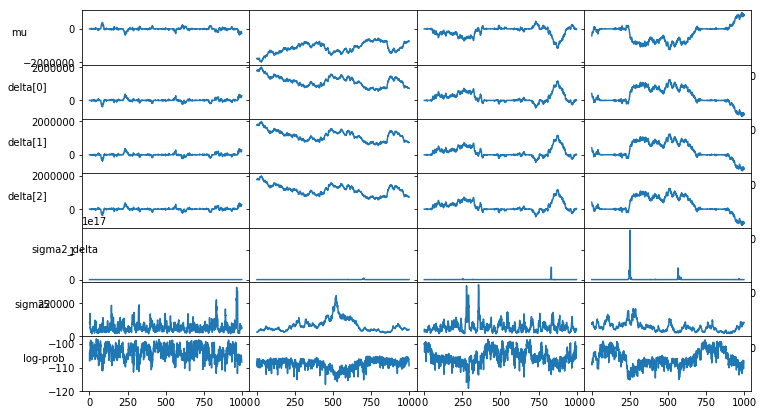
\includegraphics[width=\textwidth]{P5-chains1.png}
\end{figure}

This is not every encouraging: 1) Some chains have significantly lower log-probability. 2) $\mu$ and $\delta_g$ values strongly anti-correlate, which is an indication of non-identifiability. 3) $\sigma_\delta^2$ has incredibly large range, up to $10^{17}$ (!). All these are hallmarks of an unstable model.

To make our model more stable, we normalize the raw data, and define priors that are normalizable. This makes sure that STAN draws samples from realistic regions. To normalize the data, we calculate the empirical mean and standard deviation,
\be
	m := \frac{1}{N}\sum_g\sum_i y^\text{raw}_{g,i} = 1804.8,\qquad s := \sqrt{\frac{1}{N}\sum_g\sum_i(y^\text{raw}_{g,i} - m)^2} = 520.2,
\ee
and normalize all data points by subtracting the mean and dividing by the variance
\be
	y_{g,i} := \frac{y^\text{raw}_{g,i} - m}{s},
\ee
 $\sim 95\%$ of which will in the range $[-2.0, 2.0]$. This allows us to define plausible regions for the parameters
\ba
	\mu &=& 0,\\
	\Sigma: = \sqrt{\sigma^2 + \sigma_\delta^2} & \sim & [0.3, 3.0],\\
	\gamma: = \sigma_\delta / \Sigma &\sim & [0, 1],
\ea
where $\Sigma^2$ is the total variance, and $\gamma$ is the fraction of the total variance contributed by $\sigma_\delta^2$. We can still use a non-informative prior on $\gamma$:
\be
	P_0(\gamma) = \frac{\text{const.}}{\gamma (1- \gamma)},
\ee
but use well-defined priors for $\mu$ and $\Sigma$:
\ba
	P_0(\mu) &=& \text{Norm}(\mu\,|\,\text{mu=}0, \text{sigma=}1.0)
	\\
	P_0(\Sigma) &=& \text{Log-Norm}(\Sigma\,|\, \text{mu=}\ln(1.0),\, \text{sigma=}\frac{\ln(3.0) - \ln(0.3)}{2})
\ea

Using this new parametrization, we write run the following STAN code
\begin{lstlisting}[language={}]
data {
    int<lower=1> G;  // number of groups
    int<lower=1> N;  // total number of data points
    int<lower=1, upper=G> label[N];  // group labels
    real y[N];
}
parameters{
    real mu;  // global mean
    real delta[G];  // group deviations
    real<lower=0> Sigma;  // total variance
    real<lower=0, upper=1> gamma;  // sigma_delta^2 / Sigma^2
}
model {
    // priors
    target += normal_lpdf(mu | 0, 1.0);
    target += lognormal_lpdf(Sigma | 0, 1.151);
    target += -log(gamma) - log(1 - gamma);
    
    // likelihoods
    for (g in 1:G){
        target += normal_lpdf(delta[g] | 0, sqrt(gamma)*Sigma);
    }
    for (j in 1:N){
        target += normal_lpdf(y[j] | mu + delta[label[j]], sqrt(1-gamma)*Sigma);
    }
}
\end{lstlisting}
Running 4 chains, each with 20,000 iterations, out of which we keep only every 10th from the second half produces 4,000 samples. These are shown for the 4 chains below
\begin{figure}[h]
\centering
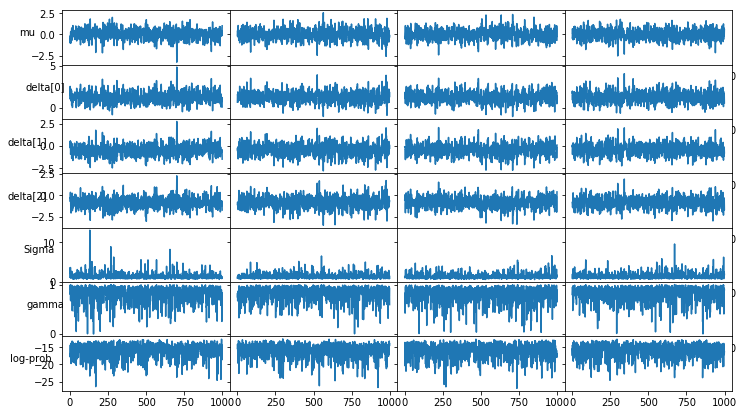
\includegraphics[width=\textwidth]{P5-chains2.png}
\end{figure}

All four chains show very similar behavior, sampled values are within realistic boundaries. STAN reports the following output
\begin{lstlisting}[language={}, numbers=none]
Inference for Stan model: anon_model_51faf35cd5be129564173392e7b29923.
4 chains, each with iter=20000; warmup=10000; thin=10; 
post-warmup draws per chain=1000, total post-warmup draws=4000.

           mean se_mean     sd   2.5%    25%    50%    75%  97.5%  n_eff   Rhat
mu       9.5e-3  9.9e-3   0.59  -1.19  -0.36 7.3e-3   0.39   1.19   3575    1.0
delta[0]   1.25    0.01   0.64   0.04   0.83   1.23   1.65   2.54   3520    1.0
delta[1]  -0.43    0.01   0.61  -1.68   -0.8  -0.42  -0.05   0.79   3682    1.0
delta[2]  -0.83    0.01   0.64  -2.13  -1.22  -0.82  -0.43    0.4   3680    1.0
Sigma      1.44    0.01   0.75   0.71   0.98   1.24   1.65   3.34   4000    1.0
gamma      0.81  2.7e-3   0.16   0.38   0.73   0.85   0.92   0.98   3439    1.0
lp__     -16.05    0.03   2.08 -21.16  -17.1 -15.64 -14.54 -13.22   4000    1.0

Samples were drawn using NUTS at Sat Apr 28 17:55:08 2018.
For each parameter, n_eff is a crude measure of effective sample size,
and Rhat is the potential scale reduction factor on split chains (at 
convergence, Rhat=1).
\end{lstlisting}

Not forgetting that these estimates are valid for the normalized data, we can obtain the estimates for the unnormalized parameters as:
\ba
	&&\mathbb{E}(\mu^\text{raw}) = m + s \times \mathbb{E}(\mu) = 1809.7,
	\qquad 
	\text{std}(\mu^\text{raw}) = s \times \text{std}(\mu)  = 308.5
	\\
	&&\mathbb{E}(\sigma_\delta^\text{raw}) = s \times \mathbb{E}(\Sigma\sqrt{\gamma} ) = 685.4, 
	\qquad
	\text{std}(\sigma_\delta^\text{raw}) = s \times \text{std}(\Sigma\sqrt{\gamma} ) = 409.1
	\\
	&&\mathbb{E}(\sigma^\text{raw}) = s \times \mathbb{E}(\Sigma\sqrt{1-\gamma} ) = 260.3, 
	\qquad
	\text{std}(\sigma^\text{raw}) = s \times \text{std}(\Sigma\sqrt{1-\gamma} ) = 71.2
	\\
	&& \mathbb{E}(\sigma^2_\delta / (\sigma_\delta^2 + \sigma^2)) = \mathbb{E}(\gamma) = 0.8056,
	\qquad 
	\text{std}(\gamma) = 0.1595.
\ea


% \subsubsection*{Problem 6 - $\exp(-x^4)$}
% In a park, the heights of 10 pine trees are measured $x = [435, 491, 620, 356, 443, 398, 383, 475, 554, 639]$ in centimeters. Assume the following distribution for the heights,
% \be
% 	P(x\,|\, c, s) = \frac{1}{Z}\frac{1}{s} \exp\left(-\frac{(x - c)^4}{s^4}\right),\qquad \text{where }Z = \frac{\Gamma(\frac{1}{4})}{2} = 1.8128,
% \ee
% and estimate the parameters $(c,s)$. [Extra: Fit a normal distribution too, and calculate which model has higher likelihood.]

% \subsubsection*{Problem 7 - Uniform}
% A pseudo-random number generator produces the following sequence $x = [8.155, 6.272, 3.583, 7.096, 6.469]$. Assume that it draws samples uniformly from an interval $l\leq x \leq h$, and estimate the parameters $(l, h)$.

% \subsubsection*{Problem 8 - Mixed error profile}
% Twelve screws produced by a machine are sent to quality control, and measured how much their length deviates from the specification. The measured deviations are $x = [$ -1.32, -8.17, -0.21, -0.73, +5.78, +1.75, -0.29, -0.34, -0.52, +1.29, -0.60, +0.28$]$ in percentages. We suspect that some unknown fraction ($f$) of the screws are affected by a much larger errors than others, and we model this mixture distribution as
% \be
% 	P(x\,|\,f, \sigma, s) = (1-f)\times\text{Normal}(x\,|\,0,\sigma) + f\times\text{Cauchy}(x\,|\,0,s) 
% 	= (1-f)\frac{1}{\sigma\sqrt{2\pi}}\exp\left(-\frac{x^2}{2\sigma^2}\right) + f \frac{1}{s\pi}\frac{1}{1 + (x/s)^2}.
% \ee
% Estimate the parameters $(f, \sigma, s)$. [Extra: For each measured deviation, estimate the probability that it is a result of the Cauchy-distributed error.] 

% \subsubsection*{Problem 9 - Multinomial}
% In an egg-processing unit, the quality control mechanism takes 20 eggs from the conveyor belt, and grades their quality, i.e. giving them labels A, B, C, D or F. The observed counts are $(n_A, n_B, n_C, n_D, n_F) = (7, 8, 3, 1, 1)$. Assuming multinomial distribution, estimate the fractions of each quality grades in this batch, i.e. the parameters $(p_A, p_B, p_C, p_D, p_F)$.

% \subsubsection*{Problem 10 - Threshold effect}
% In a school district, 3955 seniors take a new standardized math test, designed to measure the quality of math education in each school. The histogram of the scores are published, as shown below. 
% A striking feature of this data is that no students received scores below 20. This is likely an indication that the minimal passing score was 20, and grading was done in a way that ensured that no one failed. This hypothesis is supported also by the visible abundance just above the score 20. 
% \begin{figure}[h]
% \centering
% 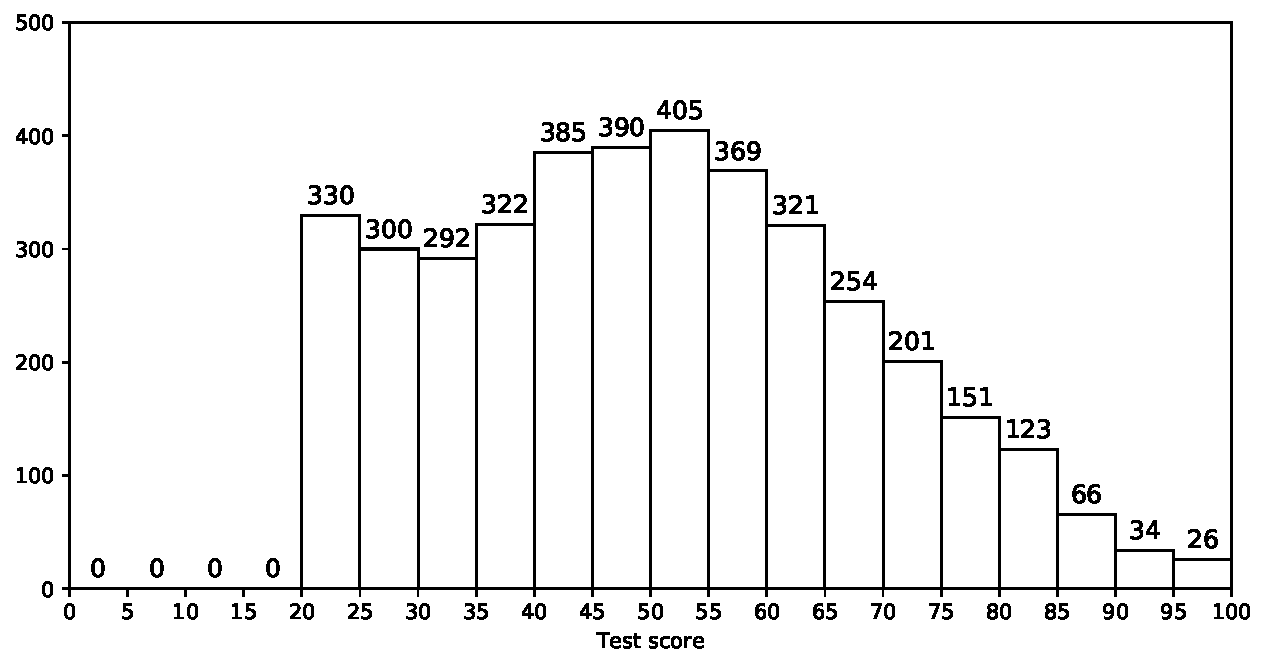
\includegraphics[width=0.6\textwidth]{test-scores.pdf}
% \end{figure}


% Let's estimate the distribution of the ``unadjusted'' scores by assuming the following process.
% \begin{itemize}
% 	\item True scores are distributed according to a normal distribution with mean $\mu$ and standard deviation $\sigma$, truncated to the $[0,100]$ interval.

% 	\item If the true score is smaller than 20, it gets adjusted. Let's model this by a replacement of the true score with an adjusted score, drawn from an exponential distribution with parameter $b$, truncated to the [20, 100] interval.
% \end{itemize}
% Estimate the parameters $(\mu, \sigma, b)$, and the proportion of the students that would have failed if their scores had not been adjusted.


\newpage
\subsection*{Appendix: Bayesian solution of linear regression}
For $N$ data points across $K$ features, i.e. $\{([X_{n,k}\,:\,k = 1,2,\ldots K], \;y_n)\,:\,n = 1,2,\ldots N\}$, the linear regression model is defined as
\be
	y_n = \left(\sum_k X_{n,k} b_k\right) + \varepsilon_n, \qquad X:\;N\times K,\quad y:\;N\times 1, \quad b:\;K\times 1,
\ee
where $\varepsilon_n \sim \text{Norm}(\cdot\,|\,0, \sigma^2)$, independent of everything else.

The likelihood can be written as
\ba
	P(y\,|\,X, b, \sigma^2) 
	&=& 
	\prod_{n=1}^{N} P(y_n\,|\,X_{n,:}, b, \sigma^2) 
	= 
	\prod_{n=1}^N \frac{1}{\sqrt{2\pi \sigma^2}} \exp\left[-\frac{(y_n - \sum_k X_{n,k}b_k)^2}{2\sigma^2}\right] \\
	&=&
	[2\pi \sigma^2]^{-\frac{N}{2}} \exp\left[-\frac{\sum_n(y_n - \sum_k X_{n,k}b_k)^2}{2\sigma^2}\right] = [2\pi \sigma^2]^{\frac{N}{2}} \exp\left[-\frac{(y - Xb)\T (y - Xb)}{2\sigma^2}\right],
\ea
where matrix-multiplication is assumed between every matrix, $X, y, b$, and $\top$ denotes transpose.

The numerator inside the exponential can be written as
\ba
	(y - Xb)\T (y - Xb) &=& \Big(b\T - y\T X (X\T X)^{-1}\Big) \underbrace{(X\T X)}_{=: N\Lambda^{-1}} \Big(b - \underbrace{(X\T X)^{-1}X\T y}_{=:\bar b}\Big) + \underbrace{y\T y - y\T X(X\T X)^{-1} X\T y}_{=: N\bar v} \\
	&=& N\left[(b - \bar b)\T \Lambda^{-1} (b - \bar b) + \bar v\right],
\ea
which shows that it is a good idea to start with computing $\Lambda, \bar b$ and $\bar v$:
\ba
	\Lambda &=& \left(\frac{1}{N}X\T X\right)^{-1}, \\ 
	\bar b &=& \frac{1}{N}\Lambda X\T y, \\
	\bar v &=& \frac{1}{N}(y - X\bar b)\T (y - X\bar b).
\ea

Let's assume a non-informative prior for $b$ and $\sigma^2$,
\be
	P_0(b,\sigma^2) = \frac{\text{const.}}{\sigma^2},
\ee
and write down the posterior
\be
	P(b,\sigma^2\,|\,y, X) = \text{const.} \times P_0(b, \sigma^2) \times P(y\,|\,X,b,\sigma^2) = \frac{1}{Z} (\sigma^2)^{-\frac{N+2}{2}} \exp\left(-\frac{N\bar v}{2\sigma^2}\right) \exp\left[-\frac{N}{2\sigma^2}(b - \bar b)\T \Lambda^{-1} (b - \bar b)\right],
\ee
the normalization constant $Z$ can be calculated by evaluating the integrals over $b$ and $\sigma^2$. 
\ba
	Z 
	&=& \intop_0^\infty\d{\sigma^2}(\sigma^2)^{-\frac{N+2}{2}} \exp\left(-\frac{N\bar v}{2\sigma^2}\right) 
	\underbrace{\intop\d{b}\exp\left[-\frac{N}{2\sigma^2}(b - \bar b)\T \Lambda^{-1} (b - \bar b)\right]}_{\left[\frac{2\pi\sigma^2}{N}\right]^{K/2}  \sqrt{\det{\Lambda}}}\\
	&=&
	\left[\frac{2\pi}{N}\right]^{\frac{K}{2}} \sqrt{\det{\Lambda}} \intop_0^{\infty}\d{\sigma^2} (\sigma^2)^{-\frac{N-K+2}{2}} \exp\left(-\frac{N\bar v}{2\sigma^2}\right) \\
	&=&
	\left[\frac{2\pi}{N}\right]^{\frac{K}{2}} \sqrt{\det{\Lambda}} \left[\frac{2}{N\bar v}\right]^{\frac{N-K}{2}} \underbrace{\intop_0^\infty\d{z} z^{\frac{N-K}{2}-1} \exp(-z)}_{\Gamma\left(\frac{N-K}{2}\right)}
\ea
Giving the normalized posterior
\be
	P(b,\sigma^2\,|\,y,X) = \frac{N^{\frac{K}{2}}}{[2\pi \sigma]^{\frac{K}{2}}\sqrt{\det{\Lambda}}} \frac{\left[\frac{N\bar v}{2}\right]^{\frac{N-K}{2}}}{\Gamma\left(\frac{N-K}{2}\right)} (\sigma^2)^{-\frac{N-K}{2}-1} \exp\left[-\frac{2\left(\frac{N\bar v}{2}\right) + (b-\bar b)\T (N\Lambda^{-1}) (b-\bar b)}{2\sigma^2}\right],
\ee
which is a multivariate normal-inverse-gamma distribution,
\be
	P(b\,|\,b_c, \alpha, \beta, V)  = \frac{1}{\sqrt{\det{V}}} [2\pi]^{-\frac{K}{2}}\frac{\beta^\alpha}{\Gamma(\alpha)} (\sigma^2)^{-\alpha - \frac{K}{2}-1} \exp\left[-\frac{2\beta + (b - b_c)\T V^{-1} (b - b_c)}{2\sigma^2}\right],
\ee
with parameters $b_c = \bar b$, $\alpha = \frac{N-K}{2}$, $\beta = \frac{N\bar v}{2}$, $V = \Lambda/N$. Mean, mode, standard deviation and correlation are
\ba
	\mathbb{E}(b) &=& \text{mode}(b) = \text{median}(b) = b_c = \bar b\\
	\mathbb{E}(\sigma^2) &=& \frac{\beta}{\alpha-1} = \frac{N\bar v}{N - K - 2},\qquad \text{mode}(\sigma^2) = \frac{\beta}{\alpha + 1} = \frac{N\bar v}{N - K + 3}\\
	\text{Var}(b) &=& \frac{\beta}{\alpha - 1} V = \frac{\bar v}{N - K -2} \Lambda \\
	\text{std}(\sigma^2) &=& \frac{\beta}{(\alpha -1)\sqrt{\alpha -2}} = \frac{\sqrt{2}N\bar v}{(N-K-2)\sqrt{N-K-4}} \\
	\text{cov}(b_k, \sigma^2) &=& 0 \quad \forall k,
\ea
where $\text{Var}(b)$ is the full covariance matrix of $b = (b_1, b_2, \ldots b_k)$.

The marginals of $\sigma^2$ and $b$ are inverse-gamma and multivariate t-distribution, respectively:
\ba
	P(\sigma^2\,|\,y, X) &=& \text{IG}(\sigma^2\,|\,\alpha, \beta) =  \frac{\beta^\alpha}{\Gamma(\alpha)} (\sigma^2)^{-\alpha-1} \exp\left(-\frac{\beta}{\sigma^2}\right)\\
	P(b\,|\,y,X) &=& \text{t-dist}(b\,|\, \nu, b_c, \Sigma) = \frac{1}{[\pi \nu]^{K/2}\sqrt{\det{\Sigma}}}\frac{\Gamma\left(\frac{\nu + K}{2}\right)}{\Gamma\left(\frac{\nu}{2}\right)} \left[1 + \frac{1}{\nu} (b - b_c)\T \Sigma^{-1} (b- b_c)\right]^{-\frac{\nu + K}{2}},
\ea
with $\alpha = \frac{N-K}{2}$, $\beta = \frac{N\bar v}{2}$, $\nu = N-K$, $b_c = \bar b$, $\Sigma = \frac{\bar v}{N-K} \Lambda$. 
Mean, std of $b_k$ and correlation between $b_k$ and $b_{k'}$ are given by
\ba
	\mathbb{E}(b_k) &=& \bar b_k \\ 
	\text{std}(b_k) &=& \sqrt{[\text{Var}(b)]_{k,k}}  = \sqrt{\frac{\bar v}{N - K - 2} \Lambda_{k,k}} \\
	\text{corr}(b_k, b_{k'}) &=& \frac{\text{cov}(b_k, b_{k'})}{\text{std}(b_k) \text{std}(b_{k'})} = \frac{\Lambda_{k,k'}}{\sqrt{\Lambda_{k,k}\Lambda_{k',k'}}}
\ea
Since $\Lambda = N (X\T X)^{-1}$, the posterior correlation between the coefficients $b_k$ is entirely determined by the combination of features present in the data, aka the design matrix $X$. 

The marginal of $b_k$ is a t-distribution with the same $\nu$ as the joint.
\be
	P(b_k\,|\,y,X) = \intop\d{b_{\neq k}} P(b\,|\,y,X)
	=
	\text{t-dist}(b_k\,|\, \nu = N-K,\, b_c = \bar{b}_k, \, \Sigma = \frac{\bar v}{N-K} \Lambda_{k,k})
\ee









\end{document}